\section{Overview}

Research on atmospheric plasmas has been going on for as long as research on
plasmas themselves. However, it was only recently that the necessary diagnostic
techniques and computational power existed to properly examine them. In the last
few decades there has been a renaissance in work dedicated to atmospheric
plasmas, particularly atmospheric pressure plasmas that are out of thermal
equilibrium. This is because they are able to treat delicate substrates with
none of the thermal damage associated with arcs.

Though several approaches exist to generating atmospheric pressure plasmas (dbd,
microwave, rf), particularly interesting are those using nanosecond pulses. The
duration of such pulses, as well as their amplitude can be changed to target
particular atomic or molecular reactions. This flexibility is highly desirable
in the world of plasma processing where selectivity, control, etc. are of utmost
importance. However, we are still learning how to measure these particular
plasmas. As recently as $1994$ \cite{Vasilyak1994} the only diagnostic with any
meaningful accuracy was propagation velocity. 

Several research groups have focused on the development of pulsed nanosecond
discharges in air. However, the complex chemistry associated with air plasmas
obscures some of the more fundamental questions: how is the pulsed nanosecond
plasma formed, how are the excited states of the system populated, what
significance is there to reactions after the fast ionization wave, the spatial
variation of system parameters, what kind of electron energy distribution can be
expected? \todo{simplify for general reader} This study will emphasize
spectroscopic measurements of a helium pulsed nanosecond discharge.

Such a system retains physical relevance given that helium is a common
stabilizing additive to atmospheric pressure plasmas. At the same time, the more
simple atomic structure lends itself to a more detailed examination using global
models, kinetic simulations, and active spectroscopy. This work will focus its
efforts on the description of the spatial variation of the pulsed-nanosecond
discharge, an approximation of its electron energy distribution function, and a
description of how the neutral atoms are excited.

The remainder of this chapter includes a review of the associated literature, as
well as a discussion of basic discharge theory (diagnostic-specific theory will
accompany the relevant chapters). Chapter \ref{chp:exp} provides the necessary
details of the experimental setup as well as some preliminary observations.
Next, in chapter \ref{chp:meta}, absolute measurements of the helium triplet
metastable densities are presented. Chapter \ref{chp:emit} covers more general
emissions measurements. In order to provide a more clear understanding of the
meaning of these measurements, we explore them using a global model and a
particle kinetics model. Finally, we conclude in chapter \ref{chp:conc} with a
discussion of how the collection of models and measurements influences our
understanding of the pulsed nanosecond discharge.

\section{Literature Review}

\subsection{History of Atmospheric-Pressure Discharges}

\todo[inline]{History of plasmas, two separate paths: arc and dbd. Thermal vs.
nonuniform. Consider how to address other, more exotic atmospheric plasmas, ie
microwave, rf, etc.}

Like most physical phenomena, plasmas are typically only described under ideal
circumstances. This means that neutral collisions, and subsequently, atmospheric
plasmas, are often ignored. Neutral collisions tend to obscure the
electromagnetic effects that distinguish a plasma from a gas. However, the
history of observation and study of plasmas is indelibly linked to atmospheric
plasmas. Lightning and static sparks are the most prevalent plasmas on earth. 
Indeed, the among the first artificial plasmas was a constant atmospheric arc
generated in $1802$, the work of a Russian scientist named Vasilii Petrov
\cite{Anders2003}.

Indeed, at present, there's a relative abundance of different
atmospheric pressure discharges: dielectric-barrier, RF, microwave, glow,
pulsed, and more. Each has unique range of parameters in which it operates, and
a survey of all possible atmospheric discharges would be excessive. Instead, we
shall focus on the two most common discharges which, together, illustrate the
distinct advantages of the nanosecond-pulsed discharge.

The work of Petrov was the forerunner to what is now referred to as the study of
thermal arcs. Such plasmas are common in industrial lighting systems, and for a
time were even used as the primary nigh-time illumination of Detroit. Perhaps
more common, is the use of thermal arcs for the welding or cutting of metals.
This potential was recognized early on. Volta's recent invention of the voltaic
pile provided the first source of constant and sufficient electrical energy.
Using a series of voltaic cells, Petrov was able to draw the first electrical
arc between two sticks of carbon. Its blinding light was recorded in a number of
historical prints, such as figure \ref{fig:humphry}.
\begin{figure}\label{fig:humphry}
  \centering
  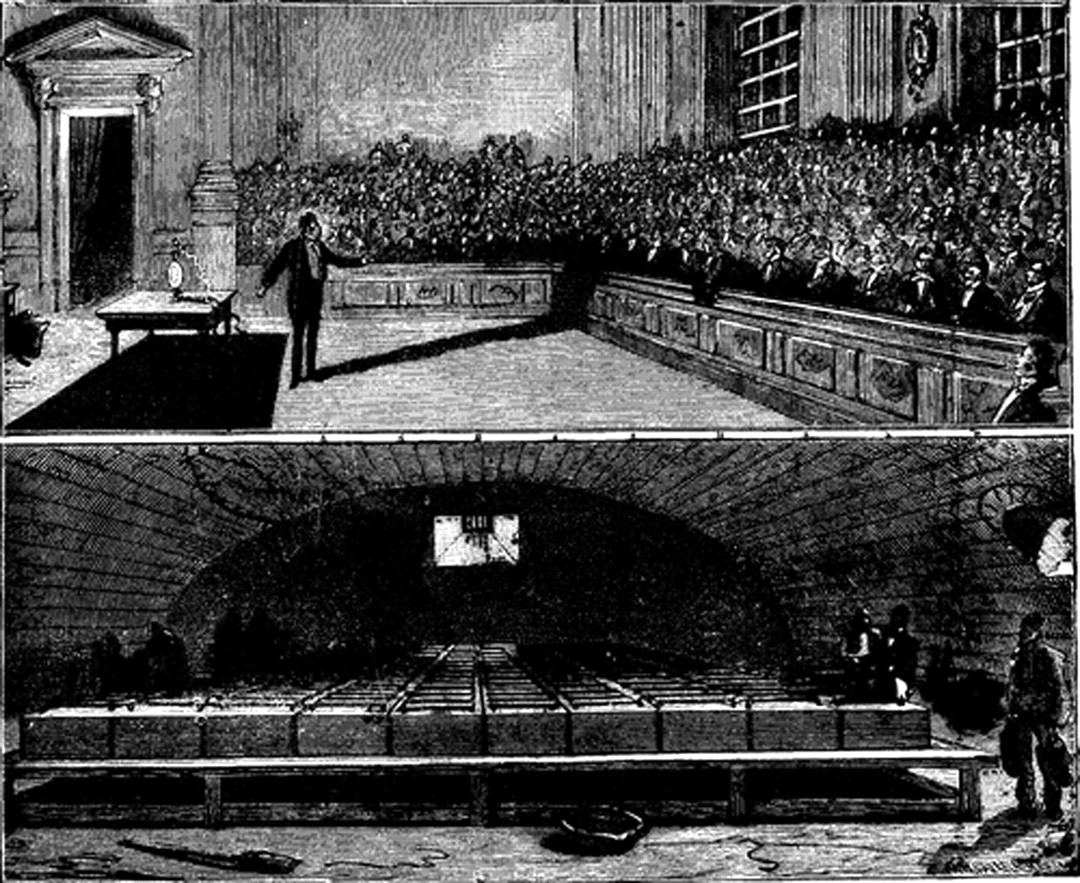
\includegraphics[scale=0.25]{chapters/introduction/figures/humphry.jpg}
  \caption{This is a test.\todo{cite}}
\end{figure}
Aside from this light, the arcs were characterized by their significant
ionization, and high degree of thermal equilibrium. Gas temperatures could reach
thousands of kelvin.

Both the primary advantage and disadvantage of thermal arcs are their high
operating temperatures. These high operating temperatures correlate with the
ability of the plasma to convert electrical energy to thermal energy; of great
values in welding or for continuum light generation. In these plasmas, some of
the energy is also converted to excited atoms or molecules. In some cases, these
species may be desirable for processing a material. However, contact with these
high temperatures will often lead to destruction of the substrate.

In contrast, later work by Werner von Siemens \cite{Siemens1857}, led to the
discovery of the so-called ``silent discharge,'' seen in figure
\ref{fig:siemens}.
\begin{figure}\label{fig:siemens}
  \centering
  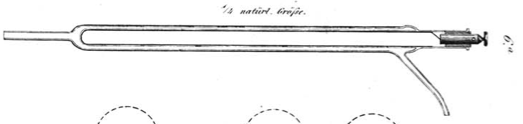
\includegraphics{chapters/introduction/figures/siemens.jpg}
  \caption{Werner von Siemens' silent discharge.\todo{cite}}
\end{figure}
In recent years, the terminology has changed and this type of
discharge is now referred to as a dielectric-barrier discharge, or \acs{dbd}.
The \acs{dbd} was significantly different from the thermal arc. Visually, it was
much dimmer, and appeared to be composed of many thousands of individual
filaments. Additionally, the \acs{dbd} did not significantly heat the air,
unlike the thermal arc. Finally, the \acs{dbd} was used in the first commercial
plasma application: ozone generation and water purification. Notably, both the
thermal arc and silent discharge predated the `official' discover of plasma by
Sir William Crookes in $1872$.

The \acs{dbd} could be used process materials. Indeed, it has become common to
use this type of discharge to treat polymer films, as well as clothes, and
medical equipment (sterilization). However, like the thermal arc, there are some
limitations. \acs{dbd}s are not particularly uniform as a result of the large
numbers of filaments. Thus, uniform processing will only occur as a result of
long processing times (when the relatively random position of these filaments is
averaged out) or if the desirable species has a long enough life to diffuse away
from where it was created. Another limitation to \acs{dbd}s is that they are
frequently generated with some sinusoidal voltage signal, at a frequency

\subsection{Repetitively-Pulsed Nanosecond Plasmas}

For a substantial period of time, these two \todo{is this true?} discharges
represented the range of atmospheric-pressure plasmas (\acs{app}). The thermal
arc, though useful, could not be used on delicate substrates. It had the
additional problem of having relatively little control over its chemical
kinetics. Meanwhile, the \acs{dbd} was relegated to ozone production and polymer
processing (relatively low-value applications). Though the \acs{dbd} had
attractive thermal properties, little else was known about how it operated, and
how to control its properties. As recently as $2007$, the National Academies
noted that ``the full promise of \acs{app}s will be known only if they can be
understood and managed based on fundamental scientific principles at two
extremes--the nanoscopic kinetic level, where selective chemistry occurs, and
the global stability level, likened to aerodynamics.''

Coincident to this work were studies of short, pulsed discharges. Initial work
by J.J. Thompson and ??? \todo{who was original?} was driven by an interest in
how breakdown occurred. As shorter pulsers were developed, a number of
researchers became interested in the characteristics of pulsed discharges
themselves. Loeb \todo{who else?} noted that the discharge properties were akin
to those observed in lightning leaders. 

\subsection{Research Plan}

Propose research to fill this gap
Specific and cited history of PNDS and related measurements.

\section{Basic Theory}

Basic theory of gaseous breakdown.
